\documentclass{article}\usepackage[]{graphicx}\usepackage[]{color}
%% maxwidth is the original width if it is less than linewidth
%% otherwise use linewidth (to make sure the graphics do not exceed the margin)
\makeatletter
\def\maxwidth{ %
  \ifdim\Gin@nat@width>\linewidth
    \linewidth
  \else
    \Gin@nat@width
  \fi
}
\makeatother

\definecolor{fgcolor}{rgb}{0.345, 0.345, 0.345}
\newcommand{\hlnum}[1]{\textcolor[rgb]{0.686,0.059,0.569}{#1}}%
\newcommand{\hlstr}[1]{\textcolor[rgb]{0.192,0.494,0.8}{#1}}%
\newcommand{\hlcom}[1]{\textcolor[rgb]{0.678,0.584,0.686}{\textit{#1}}}%
\newcommand{\hlopt}[1]{\textcolor[rgb]{0,0,0}{#1}}%
\newcommand{\hlstd}[1]{\textcolor[rgb]{0.345,0.345,0.345}{#1}}%
\newcommand{\hlkwa}[1]{\textcolor[rgb]{0.161,0.373,0.58}{\textbf{#1}}}%
\newcommand{\hlkwb}[1]{\textcolor[rgb]{0.69,0.353,0.396}{#1}}%
\newcommand{\hlkwc}[1]{\textcolor[rgb]{0.333,0.667,0.333}{#1}}%
\newcommand{\hlkwd}[1]{\textcolor[rgb]{0.737,0.353,0.396}{\textbf{#1}}}%
\let\hlipl\hlkwb

\usepackage{framed}
\makeatletter
\newenvironment{kframe}{%
 \def\at@end@of@kframe{}%
 \ifinner\ifhmode%
  \def\at@end@of@kframe{\end{minipage}}%
  \begin{minipage}{\columnwidth}%
 \fi\fi%
 \def\FrameCommand##1{\hskip\@totalleftmargin \hskip-\fboxsep
 \colorbox{shadecolor}{##1}\hskip-\fboxsep
     % There is no \\@totalrightmargin, so:
     \hskip-\linewidth \hskip-\@totalleftmargin \hskip\columnwidth}%
 \MakeFramed {\advance\hsize-\width
   \@totalleftmargin\z@ \linewidth\hsize
   \@setminipage}}%
 {\par\unskip\endMakeFramed%
 \at@end@of@kframe}
\makeatother

\definecolor{shadecolor}{rgb}{.97, .97, .97}
\definecolor{messagecolor}{rgb}{0, 0, 0}
\definecolor{warningcolor}{rgb}{1, 0, 1}
\definecolor{errorcolor}{rgb}{1, 0, 0}
\newenvironment{knitrout}{}{} % an empty environment to be redefined in TeX

\usepackage{alltt}
\usepackage[utf8]{inputenc}
\usepackage{ngerman}
\usepackage{hyperref}
\usepackage{graphicx}

% Article setup --------------------------------------------
\title{Einführung in die Datenanalyse mit $\mathcal{R}$\newline%
  Weiterführende Hinweise%
}
% \subtitle{Weiterführende Hinweise}
\author{
  Dag Tanneberg\thanks{
    \href{mailto:dag.tanneberg@uni-potsdam.de}{dag.tanneberg@uni-potsdam.de}
  }
}
\date{\today}

% Hyperlink setup
% \hypersetup{colorlinks, urlcolor = red, linkcolor = }
\IfFileExists{upquote.sty}{\usepackage{upquote}}{}
\begin{document}
\maketitle



\section{Auswertung multiplikativer Interaktionsterme}

Die letzte Sitzung der Veranstaltung riss die Schätzung und
Auswertung generalisierter linearer Modelle (GLM) an. Die
Illustration griff auf einen Datensatz zurück, der Informationen
über alle namentlich erwähnten Charaktere der Fantasyreihe ``A
Song of Ice and Fire'' bereitstellte. Die Fragestellung lautete,
mit welcher Wahrscheinlichkeit der Hauptcharakter Jon Snow sterben
würde. Zu ihrer Beantwortung griff die Veranstaltung auf Angaben
über die Zugehörigkeit zu einem Adelshaus, das Alter\footnote{
  In Ermangelung besserer Informationen misst die entsprechende
  Variable nicht das natürliche Alter, sondern zählt die Anzahl
  der seit Einführung des Character verstrichenen Kapitel. Mit
  etwas gutem Willen handelt es sich um eine Messung der
  Prozesszeit.
},
das Geschlecht sowie den Adelsstatus zurück. Das
vorgeschlagene logistische Regressionsmodell beinhaltete außerdem
eine Interaktion von Geschlecht und Adelsstatus sowie ein
kubisches Polynom des Alters. Offen blieb zum Schluss die
Auswertung multiplikativer Interaktionsterme. Dieser Abschnitt
demonstriert eine Strategie zur die graphische Auswertung
entsprechender Terme.

Zunächst sei an das Regressionsmodell erinnert, mit dessen Hilfe


\begin{knitrout}
\definecolor{shadecolor}{rgb}{0.969, 0.969, 0.969}\color{fgcolor}\begin{kframe}
\begin{alltt}
\hlstd{fit} \hlkwb{<-} \hlkwd{glm}\hlstd{(} \hlcom{# generate model}
  \hlstd{died} \hlopt{~} \hlnum{0} \hlopt{+} \hlstd{allegiances} \hlopt{+}
    \hlstd{gender}\hlopt{*}\hlstd{nobility} \hlopt{+}
    \hlstd{age_in_chapters} \hlopt{+} \hlkwd{I}\hlstd{(age_in_chapters}\hlopt{^}\hlnum{2}\hlstd{)} \hlopt{+} \hlkwd{I}\hlstd{(age_in_chapters}\hlopt{^}\hlnum{3}\hlstd{),}
  \hlkwc{family} \hlstd{=} \hlkwd{binomial}\hlstd{(}\hlkwc{link} \hlstd{=} \hlstr{"logit"}\hlstd{),}
  \hlkwc{data} \hlstd{= asoiaf}
\hlstd{)}
\end{alltt}
\end{kframe}
\end{knitrout}

Multiplikative Interaktionsterme können in verschiedenen
Formen ausgewertet werden. In den Sozialwissenschaften
erfreuen sich sogenannte Marginal Effect Plots besonderer
Beliebtheit und sie treten in verschiedenen Varianten auf.

\begin{enumerate}
  \item Darstellung der partiellen Ableitung
  \item Darstellung der
\end{enumerate}


\begin{knitrout}
\definecolor{shadecolor}{rgb}{0.969, 0.969, 0.969}\color{fgcolor}\begin{kframe}
\begin{alltt}
\hlstd{pred_data} \hlkwb{<-} \hlkwd{expand.grid}\hlstd{(}
  \hlkwc{allegiances} \hlstd{=} \hlkwd{c}\hlstd{(}\hlstr{"Baratheon"}\hlstd{,}  \hlstr{"Lannister"}\hlstd{,} \hlstr{"Stark"}\hlstd{,} \hlstr{"Targaryen"}\hlstd{),}
  \hlkwc{nobility} \hlstd{=} \hlnum{0}\hlopt{:}\hlnum{1}\hlstd{,} \hlkwc{gender} \hlstd{=} \hlnum{0}\hlopt{:}\hlnum{1}\hlstd{,}
  \hlkwc{age_in_chapters} \hlstd{=} \hlkwd{median}\hlstd{(asoiaf[,} \hlstr{"age_in_chapters"}\hlstd{],} \hlkwc{na.rm} \hlstd{=} \hlnum{TRUE}\hlstd{),}
  \hlkwc{stringsAsFactors} \hlstd{=} \hlnum{FALSE}
\hlstd{)}
\end{alltt}
\end{kframe}
\end{knitrout}

Der resultierende Datensatz enthält eine Zeile für jede der
vier möglichen Kombinationen von \textbf{gender} und
\textbf{nobility}. Die werte der Variablen \textbf{allegiances}
und \textbf{age{\textunderscore}in{\textunderscore}chapters}
bleiben über alle Reihen hinweg konstant.

\begin{knitrout}
\definecolor{shadecolor}{rgb}{0.969, 0.969, 0.969}\color{fgcolor}\begin{kframe}
\begin{verbatim}
##    allegiances nobility gender age_in_chapters
## 1    Baratheon        0      0             126
## 2    Lannister        0      0             126
## 3        Stark        0      0             126
## 4    Targaryen        0      0             126
## 5    Baratheon        1      0             126
## 6    Lannister        1      0             126
## 7        Stark        1      0             126
## 8    Targaryen        1      0             126
## 9    Baratheon        0      1             126
## 10   Lannister        0      1             126
## 11       Stark        0      1             126
## 12   Targaryen        0      1             126
## 13   Baratheon        1      1             126
## 14   Lannister        1      1             126
## 15       Stark        1      1             126
## 16   Targaryen        1      1             126
\end{verbatim}
\end{kframe}
\end{knitrout}

Mit Hilfe der Funktion \textbf{predict()}

\begin{knitrout}
\definecolor{shadecolor}{rgb}{0.969, 0.969, 0.969}\color{fgcolor}\begin{kframe}
\begin{alltt}
\hlstd{pred_data[,} \hlstr{"fitted"}\hlstd{]} \hlkwb{<-} \hlkwd{predict}\hlstd{(fit,} \hlkwc{newdata} \hlstd{= pred_data,} \hlkwc{type} \hlstd{=} \hlstr{"response"}\hlstd{)}
\hlstd{pred_data}
\end{alltt}
\begin{verbatim}
##    allegiances nobility gender age_in_chapters     fitted
## 1    Baratheon        0      0             126 0.35480247
## 2    Lannister        0      0             126 0.30433574
## 3        Stark        0      0             126 0.39193082
## 4    Targaryen        0      0             126 0.05682782
## 5    Baratheon        1      0             126 0.10427826
## 6    Lannister        1      0             126 0.08476429
## 7        Stark        1      0             126 0.12006921
## 8    Targaryen        1      0             126 0.01259482
## 9    Baratheon        0      1             126 0.30551914
## 10   Lannister        0      1             126 0.25924574
## 11       Stark        0      1             126 0.34020963
## 12   Targaryen        0      1             126 0.04598431
## 13   Baratheon        1      1             126 0.36266208
## 14   Lannister        1      1             126 0.31161734
## 15       Stark        1      1             126 0.40010286
## 16   Targaryen        1      1             126 0.05868707
\end{verbatim}
\end{kframe}
\end{knitrout}

\begin{knitrout}
\definecolor{shadecolor}{rgb}{0.969, 0.969, 0.969}\color{fgcolor}\begin{kframe}
\begin{alltt}
\hlstd{pred_data} \hlkwb{<-} \hlkwd{within}\hlstd{(pred_data, \{}
  \hlcom{# Note: within() requires curly brackets whenever you want to}
  \hlcom{# evaluate multiple statements.}
  \hlstd{gender_label} \hlkwb{<-} \hlkwd{factor}\hlstd{(gender,} \hlnum{0}\hlopt{:}\hlnum{1}\hlstd{,} \hlkwd{c}\hlstd{(}\hlstr{"Female"}\hlstd{,} \hlstr{"Male"}\hlstd{))}
  \hlstd{nobility_label} \hlkwb{<-} \hlkwd{factor}\hlstd{(nobility,} \hlnum{0}\hlopt{:}\hlnum{1}\hlstd{,} \hlkwd{c}\hlstd{(}\hlstr{"Commoner"}\hlstd{,} \hlstr{"Noble"}\hlstd{))}
  \hlstd{\}}
\hlstd{)}
\hlkwd{ggplot}\hlstd{(}
  \hlkwc{data} \hlstd{= pred_data,}
  \hlkwc{mapping} \hlstd{=} \hlkwd{aes}\hlstd{(}\hlkwc{x} \hlstd{= allegiances,} \hlkwc{y} \hlstd{= fitted,} \hlkwc{fill} \hlstd{= gender_label)}
\hlstd{)} \hlopt{+}
  \hlkwd{geom_bar}\hlstd{(}\hlkwc{stat} \hlstd{=} \hlstr{'identity'}\hlstd{,} \hlkwc{position} \hlstd{=} \hlstr{"dodge"}\hlstd{)} \hlopt{+}
  \hlkwd{facet_grid}\hlstd{(} \hlopt{~} \hlstd{nobility_label)} \hlopt{+}
  \hlkwd{labs}\hlstd{(}
    \hlkwc{title} \hlstd{=} \hlstr{"Interaction of Gender and Nobility"}\hlstd{,}
    \hlkwc{x} \hlstd{=} \hlstr{""}\hlstd{,}
    \hlkwc{y} \hlstd{=} \hlstr{"Expected probability of death"}\hlstd{,}
    \hlkwc{fill} \hlstd{=} \hlstr{"Gender"}
  \hlstd{)} \hlopt{+}
  \hlkwd{theme}\hlstd{(}\hlkwc{legend.position} \hlstd{=} \hlstr{"bottom"}\hlstd{)}
\end{alltt}
\end{kframe}

{\centering 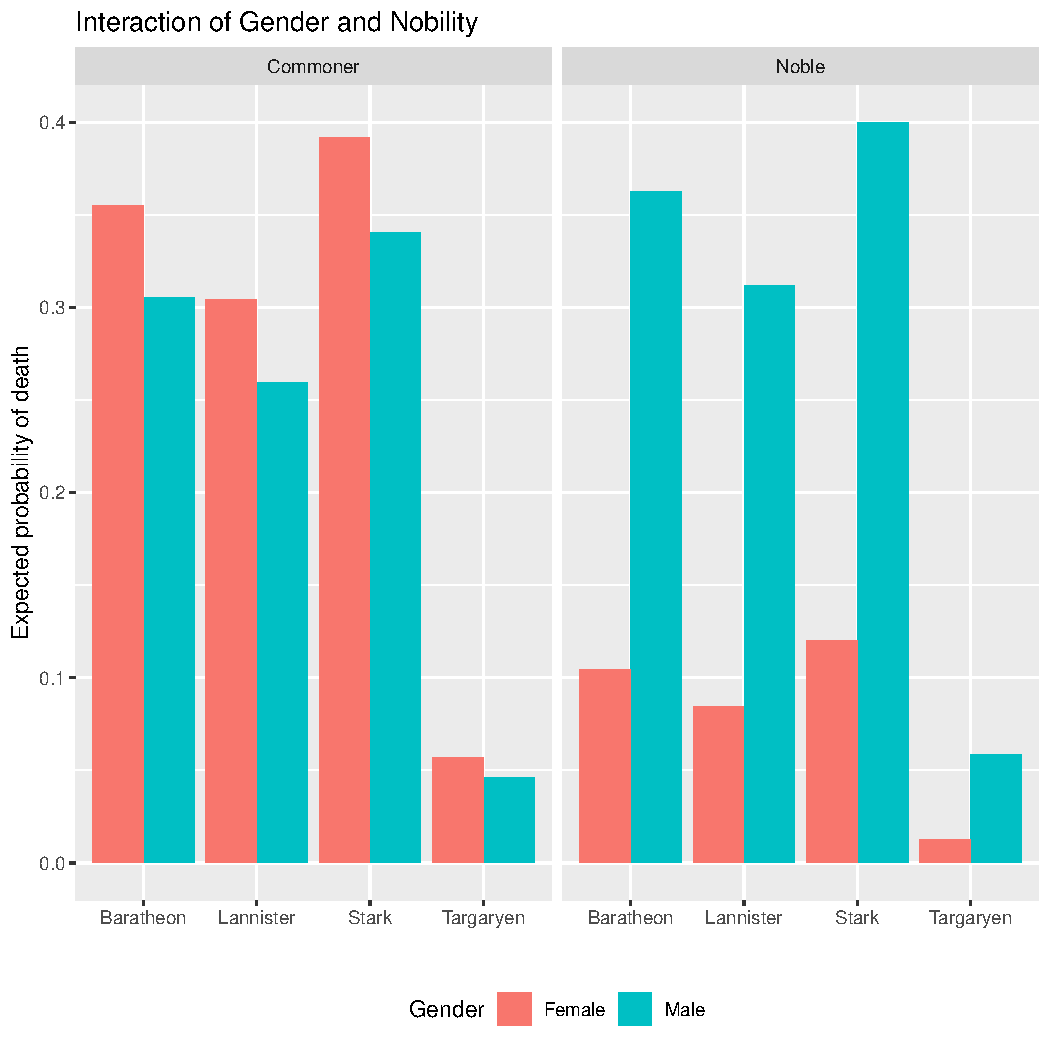
\includegraphics[width=\maxwidth]{figure/generateMarginalEffectsPlot-1} 

}



\end{knitrout}

Häufig verwenden die Sozialwissenschaften Marginal Effect Plots,
d.\,h. grafische Darstellungen der slope.

\begin{knitrout}
\definecolor{shadecolor}{rgb}{0.969, 0.969, 0.969}\color{fgcolor}\begin{kframe}
\begin{alltt}
\hlstd{fit2} \hlkwb{<-} \hlkwd{glm}\hlstd{(} \hlcom{# generate model}
  \hlstd{died} \hlopt{~} \hlnum{0} \hlopt{+} \hlstd{allegiances} \hlopt{+}
    \hlstd{gender} \hlopt{+} \hlstd{nobility} \hlopt{*} \hlstd{age_in_chapters,}
  \hlkwc{family} \hlstd{=} \hlkwd{binomial}\hlstd{(}\hlkwc{link} \hlstd{=} \hlstr{"logit"}\hlstd{),}
  \hlkwc{data} \hlstd{= asoiaf}
\hlstd{)}
\hlkwd{summary}\hlstd{(fit2)}
\end{alltt}
\begin{verbatim}
## 
## Call:
## glm(formula = died ~ 0 + allegiances + gender + nobility * age_in_chapters, 
##     family = binomial(link = "logit"), data = asoiaf)
## 
## Deviance Residuals: 
##     Min       1Q   Median       3Q      Max  
## -2.7193  -0.5640  -0.2196   0.5709   3.0360  
## 
## Coefficients:
##                           Estimate Std. Error z value Pr(>|z|)    
## allegiancesArryn          0.681880   0.732736   0.931  0.35206    
## allegiancesBaratheon      2.421455   0.531316   4.557 5.18e-06 ***
## allegiancesGreyjoy        0.677669   0.452667   1.497  0.13438    
## allegiancesLannister      2.060059   0.466747   4.414 1.02e-05 ***
## allegiancesMartell       -0.121929   0.713560  -0.171  0.86432    
## allegiancesNight's Watch  3.067868   0.506599   6.056 1.40e-09 ***
## allegiancesNone           1.127318   0.350692   3.215  0.00131 ** 
## allegiancesStark          2.378484   0.430761   5.522 3.36e-08 ***
## allegiancesTargaryen      0.151837   0.575078   0.264  0.79176    
## allegiancesTully          1.914210   0.660467   2.898  0.00375 ** 
## allegiancesTyrell         0.713196   0.878618   0.812  0.41695    
## allegiancesWildling       2.155148   0.487756   4.418 9.94e-06 ***
## gender                    0.604277   0.293921   2.056  0.03979 *  
## nobility                 -1.395722   0.331915  -4.205 2.61e-05 ***
## age_in_chapters          -0.026748   0.002422 -11.046  < 2e-16 ***
## nobility:age_in_chapters  0.012813   0.002899   4.421 9.84e-06 ***
## ---
## Signif. codes:  0 '***' 0.001 '**' 0.01 '*' 0.05 '.' 0.1 ' ' 1
## 
## (Dispersion parameter for binomial family taken to be 1)
## 
##     Null deviance: 1243.51  on 897  degrees of freedom
## Residual deviance:  666.25  on 881  degrees of freedom
##   (20 observations deleted due to missingness)
## AIC: 698.25
## 
## Number of Fisher Scoring iterations: 6
\end{verbatim}
\end{kframe}
\end{knitrout}



\end{document}
